\section{Event-driven Burst Buffer Simulator}

We develop an event-driven simulator for burst buffer enabled HPC system, named \textbf{BBSim},
from scratch in Python to mimic Cerberus scheduling Trinity.
It roughly consists of 1,400 lines of code.
Figure~\ref{Fig:JobFSM} depicts the simulation lifetime of a job in BBSim.
The \textit{state} of the job changes depends on its current status and
happening \textit{events}, along with which an \textit{action} is taken.
For example, submitted $job_i$ will enter \textbf{Wait Stage-in} state;
this state transition triggers Cerberus doing scheduling.
If $job_i$ scheduled to do stage-in, it changes to Staging-in state
and is removed from the input queue $Q_I$;
otherwise, $Q_I$ will hold $job_i$ and its status remains unchanged.
When required data is loaded into burst buffer, $job_i$ will be put into $Q_R$;
when data is ready on compute nodes' memory,
Cerberus releases the burst buffer previously taken up by $job_i$ and schedules $Q_I$.
In addition to submission, whenever system resources are released,
Cerberus will exam and schedule on corresponding queues.

There are generally two types of events in BBSim:
For those jobs selected by Cerberus,
we generate ``finish stage-in/run/stage-out'' event after
they are removed from $Q_I$/$Q_R$/$Q_O$.
The timestamps of these events are calculated using following model:
\begin{align}
        TS_{fin\_in} &= TS_{start\_in} + \frac{bb\_in}{BW_{io\_to\_bb}}\label{Equ:FinIn} \\
        TS_{fin\_run} &= TS_{fin\_mem\_in} + \frac{bb\_run}{BW_{cn\_to\_bb}}\label{Equ:FinRun} \\
        TS_{fin\_out} &= TS_{fin\_mem\_out} + \frac{bb\_out}{BW_{bb\_to\_io}} \label{Equ:FinOut}
\end{align}
where $TS_{fin\_x}$ stands for the timestamps of finishing phase $x$,
$TS_{start\_x}$ stands for the timestamps of starting phase $x$,
$TS_{fin\_mem\_x}$ stands for the timestamps of memory related input/output.
BBSim generates resource-release events
according to our model described in Section~\ref{Sec:scheduler}.
That is, at $TS_{fin\_mem\_in}$, burst buffer nodes allocated in phase 1 can be released;
\begin{align}
        TS_{fin\_mem\_in} &= TS_{start\_run} + \frac{bb\_in}{BW_{bb\_to\_cn}}\label{Equ:FinMemIn} \\
        TS_{fin\_mem\_out} &= TS_{start\_out} + \frac{bb\_out}{BW_{cn\_to\_bb}}\label{Equ:FinMemOut} \\
\end{align}

Notice Equation~\ref{Equ:FinRun} assumes that the bandwidth from compute nodes to
burst buffer nodes and the bandwidth from the other way around are the same.
BBSim does not need to generate events like ``not scheduled'',
``staging in/out data'', and ``running''.

Though target on burst buffer system, BBSim supports simulating system with only
traditional IO nodes.
It is not coupled with Cerberus; it is easy to simulating many other scheduler in BBSim,
which can be proved by our following experiments for various schedulers.

\begin{figure}[!t]
        \centering
        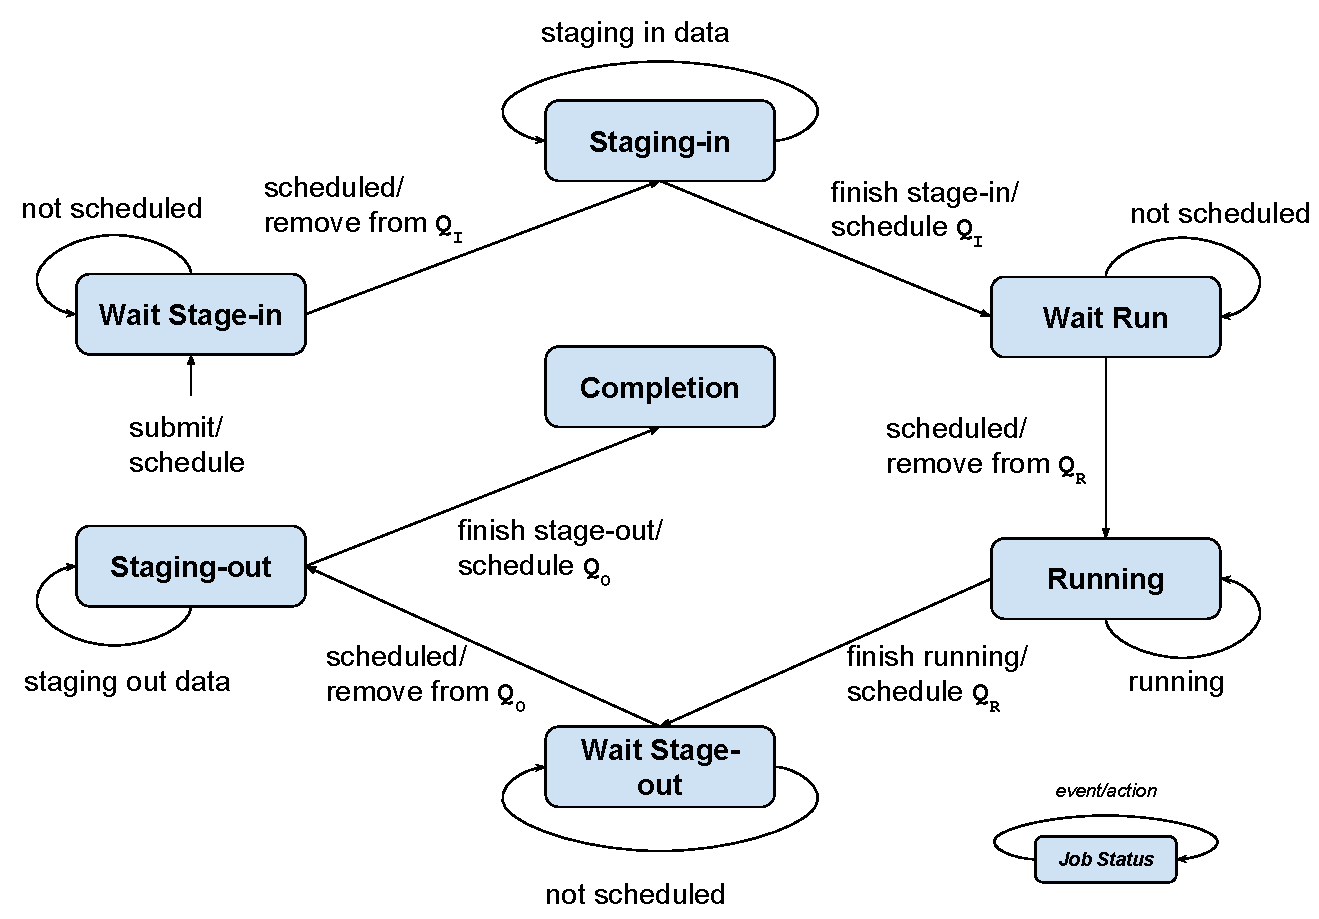
\includegraphics[width=3.5in]{3PhaseJobFSM}
        \caption{Finite State Machine of Scheduling Simulation}
        \label{Fig:JobFSM}
\end{figure}


